\section{Introduction}
\label{sec:intro}

Drafting in \mtg{} is a sequential game of imperfect information: eight
players pass packs of cards, each privately assembling a deck one pick at a
time. Strong pick models exist. Supervised models trained on human draft
logs reach 48.7--71\% agreement with human picks within a
set~\citep{ward2021drafting,czerner2025puder,brooks2024statistical} (a
general, not expert-filtered, pick population; experts are easier to
predict, scoring several points higher), but
they are set-specific. Each model encodes cards as vocabulary indices,
learns from picks made in that set, and transfers nowhere. Because public
draft logs appear on a delay, a data-driven assistant for a new set cannot
exist until roughly two weeks after release~\citep{brooks2024statistical}.
On release day, the state of the art is a spreadsheet of hand-tuned expert
ratings~\citep{draftsimratings}.

This paper asks how far pure transfer can go. DraftFM is a single pick
model trained across every public \seventeenlands{} draft set. To DraftFM,
a card is nothing but a frozen vector of public information: structured
features parsed from its Scryfall record, plus a sentence embedding of its
rules text. The model has no set-identity parameters and no per-card
weights. Whatever it knows about a set it must infer from the cards in the
pack and the drafter's accumulating pool, not from a memorized identity.
That inference transfers to a set released tomorrow. A memorized card
vocabulary cannot.

A model like this invites an obvious failure mode: report a number that
was quietly tuned on the very test set it claims never to have seen. We
designed the evaluation against exactly that risk. The protocol
(\S\ref{sec:protocol}) was frozen in a tagged public commit before the test
set existed. That test set is MSH, a licensed-IP set whose public draft
data had not yet been published at the freeze. No training, tuning, or
metric choice touches MSH pick data; the headline number comes from a
single pre-registered inference pass over the first public snapshot. All
model-selection decisions instead happen on three development sets, BRO,
TMT, and SOS, held out of training. We chose that trio so our numbers are
directly comparable to the only published multi-set zero-shot benchmark
built on public features~\citep{bertram2024cards} (same BRO holdout) and to
our own strongest per-set models.

On the development trio, DraftFM agrees with expert picks \FdevDevMean\%
of the time (\FdevBro\% / \FdevTmt\% / \FdevSos\% on BRO / TMT / SOS). To
read that number, it helps to know the best any model can do on one of
these sets: train a model directly on the set, so it actually sees the
set's own picks. That directly-trained model marks the ceiling. DraftFM,
despite training on zero picks from the target set, reaches
\NormScoreDevMean\% of that ceiling (the pre-registered normalized score,
identical held-out picks, \S\ref{sec:protocol}).

DraftFM also clears every published number we could find that a real
deployment could have used on release day. Three reference points: an
expert-tuned rating system at 44.5\%~\citep{ward2021drafting} on M19; an
hour-zero rarity heuristic at \BaseRarity\% (measured on SOS as a rehearsal
stand-in, not per dev set); and zero-shot GPT-4o at
43\%~\citep{bertram2025urzagpt} on NEO. Each of these numbers comes from a
different test set than DraftFM's, so Table~\ref{tab:baselines} presents
them as reference points rather than a head-to-head ranking. The one
comparison that does share a test set is the rarity heuristic against
DraftFM's own SOS number (\FdevSos\%). On MSH itself, the frozen evaluation
gives \FfullMsh\% expert top-1 agreement.

Contributions:
\begin{itemize}
  \item \textbf{A cross-set model and recipe.} A two-tower architecture
  over frozen card features. A pre-registered comparison tests a
  \FdevParams M-parameter design that also reads the full set's card list
  against a simpler \FfullParams M-parameter version that drops that
  component; the simpler version wins and is what ships (we call it
  A-noctx, \S\ref{sec:analysis}). It trains on \FdevPicks M picks in about
  \FdevWallHours{} hours on a single consumer workstation
  (\S\ref{sec:method}).
  \item \textbf{A frozen zero-shot benchmark.} A pre-registered,
  tamper-evident protocol for day-one draft evaluation, plus the first
  multi-set zero-shot numbers that use no post-release information of any
  kind (\S\ref{sec:protocol}, \S\ref{sec:results}).
  \item \textbf{A scaling study.} Zero-shot accuracy as a function of
  training-set count from 1 to \FdevSets{} sets, with set-composition
  probes and zero-shot seed bands at two rungs (\S\ref{sec:results}; the
  bands bound the curve's seed noise rather than fully characterize it,
  see caveat there).
  \item \textbf{A licensed-IP shift analysis.} Pre-registered experiments
  that isolate what text embeddings contribute when a set's names and
  flavor come from a licensed universe rather than in-universe \mtg{}
  (\S\ref{sec:analysis}).
  \item \textbf{Release.} Code, the frozen protocol, data manifests, model
  weights, and per-pick prediction files for every number in this paper
  (Appendix~\ref{sec:repro}).
\end{itemize}

\begin{figure}[t]
\centering
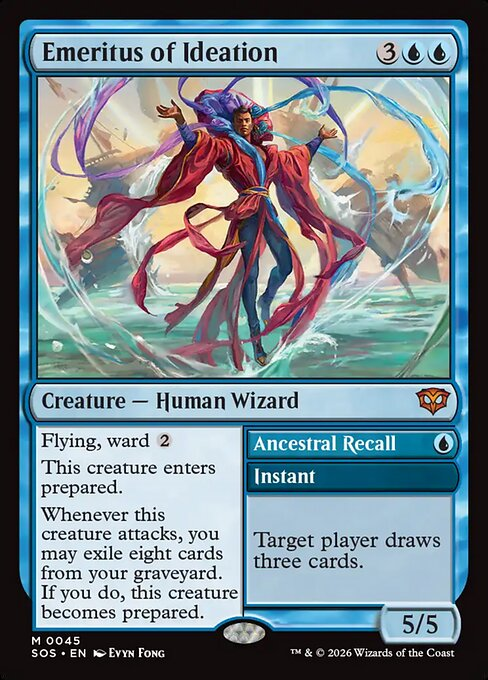
\includegraphics[width=0.24\linewidth]{figures/cards/emeritus-of-ideation.jpg}
\caption{Emeritus of Ideation, an actual first pick from a real thirteen-card
SOS pack (empty pool). The per-set ceiling model (Table~\ref{tab:main})
ranks it above every other card in the pack by a wide margin: real
expected value\protect\footnotemark{} \VHeroEv, seen in \VHeroGih{} of games it's
in, average last-seen-at pick \VHeroAlsa, and \VHeroDominance{} model
dominance over the closest candidate in the pack (\VHeroRunnerOneName).
SOS is a public development set, never the frozen MSH test set
(\S\ref{sec:protocol}); this figure illustrates the model's output, not a
headline result. Numbers regenerated by
\texttt{figures/make\_verdict\_panels.py}.}
\label{fig:teaser}
\end{figure}
\footnotetext{\emph{Expected value} is this per-set model's own raw score
for the card (higher is better; not a model input, and not the top-1
agreement metric reported elsewhere in this paper). \emph{GIH\%} and
\emph{ALSA} are \seventeenlands{} per-card statistics reported for
context: GIH\% is win rate in games where the card was drawn, and ALSA is
the average pick number at which the card was last seen (lower means
drafters value it more highly). \emph{Model dominance} is this paper's
own pairwise measure, $\mathrm{sigmoid}(\text{top EV} - \text{runner-up
EV})$.}
\FloatBarrier
